\documentclass{article}
% Change "article" to "report" to get rid of page number on title page
\usepackage{amsmath,amsfonts,amsthm,amssymb}
\usepackage{setspace}
\usepackage{Tabbing}
\usepackage{fancyhdr}
\usepackage{lastpage}
\usepackage{extramarks}
\usepackage{chngpage}
\usepackage{soul,color}
\usepackage{graphicx,float,wrapfig}
\usepackage{multirow,multicol,alltt}
\usepackage{enumerate}
% In case you need to adjust margins:
\topmargin=-0.45in      %
\evensidemargin=0in     %
\oddsidemargin=0in      %
\textwidth=6.5in        %
\textheight=9.0in       %
\headsep=0.25in         %

% Homework Specific Information
\newcommand{\hmwkTitle}{Rethinking about ME algorithm}
\newcommand{\hmwkClass}{}
\newcommand{\hmwkAuthorName}{Donglai\ Wei}


% Setup the header and footer
\pagestyle{fancy}                                                       %
\lhead{\hmwkAuthorName}                                                 %
\rhead{\firstxmark}                                                     %
\lfoot{\lastxmark}                                                      %
\cfoot{}                                                                %
\rfoot{Page\ \thepage\ of\ \pageref{LastPage}}                          %
\renewcommand\headrulewidth{0.4pt}                                      %
\renewcommand\footrulewidth{0.4pt}                                      %

% This is used to trace down (pin point) problems
% in latexing a document:
%\tracingall

%%%%%%%%%%%%%%%%%%%%%%%%%%%%%%%%%%%%%%%%%%%%%%%%%%%%%%%%\begin{enumerate}

% Some tools
\newcommand{\enterProblemHeader}[1]{\nobreak\extramarks{#1}{#1 continued on next page\ldots}\nobreak%
                                    \nobreak\extramarks{#1 (continued)}{#1 continued on next page\ldots}\nobreak}%
\newcommand{\exitProblemHeader}[1]{\nobreak\extramarks{#1 (continued)}{#1 continued on next page\ldots}\nobreak%
                                   \nobreak\extramarks{#1}{}\nobreak}%

\newlength{\labelLength}
\newcommand{\labelAnswer}[2]
  {\settowidth{\labelLength}{#1}%
   \addtolength{\labelLength}{0.25in}%
   \changetext{}{-\labelLength}{}{}{}%
   \noindent\fbox{\begin{minipage}[c]{\columnwidth}#2\end{minipage}}%
   \marginpar{\fbox{#1}}%

   % We put the blank space above in order to make sure this
   % \marginpar gets correctly placed.
   \changetext{}{+\labelLength}{}{}{}}%

\setcounter{secnumdepth}{0}
\newcommand{\homeworkProblemName}{}%
\newcounter{homeworkProblemCounter}%
\newenvironment{homeworkProblem}[1][Problem \arabic{homeworkProblemCounter}]%
  {\stepcounter{homeworkProblemCounter}%
   \renewcommand{\homeworkProblemName}{#1}%
   \section{\homeworkProblemName}%
   \enterProblemHeader{\homeworkProblemName}}%
  {\exitProblemHeader{\homeworkProblemName}}%

\newcommand{\problemAnswer}[1]
  {\noindent\fbox{\begin{minipage}[c]{\columnwidth}#1\end{minipage}}}%

\newcommand{\problemLAnswer}[1]
  {\labelAnswer{\homeworkProblemName}{#1}}

\newcommand{\homeworkSectionName}{}%
\newlength{\homeworkSectionLabelLength}{}%
\newenvironment{homeworkSection}[1]%
  {% We put this space here to make sure we're not connected to the above.
   % Otherwise the changetext can do funny things to the other margin

   \renewcommand{\homeworkSectionName}{#1}%
   \settowidth{\homeworkSectionLabelLength}{\homeworkSectionName}%
   \addtolength{\homeworkSectionLabelLength}{0.25in}%
   \changetext{}{-\homeworkSectionLabelLength}{}{}{}%
   \subsection{\homeworkSectionName}%
   \enterProblemHeader{\homeworkProblemName\ [\homeworkSectionName]}}%
  {\enterProblemHeader{\homeworkProblemName}%

   % We put the blank space above in order to make sure this margin
   % change doesn't happen too soon (otherwise \sectionAnswer's can
   % get ugly about their \marginpar placement.
   \changetext{}{+\homeworkSectionLabelLength}{}{}{}}%

\newcommand{\sectionAnswer}[1]
  {% We put this space here to make sure we're disconnected from the previous
   % passage

   \noindent\fbox{\begin{minipage}[c]{\columnwidth}#1\end{minipage}}%
   \enterProblemHeader{\homeworkProblemName}\exitProblemHeader{\homeworkProblemName}%
   \marginpar{\fbox{\homeworkSectionName}}%

   % We put the blank space above in order to make sure this
   % \marginpar gets correctly placed.
   }%

%%%%%%%%%%%%%%%%%%%%%%%%%%%%%%%%%%%%%%%%%%%%%%%%%%%%%%%%%%%%%



%%%%%%%%%%%%%%%%%%%%%%%%%%%%%%%%%%%%%%%%%%%%%%%%%%%%%%%%%%%%%
% Make title
\title{\vspace{0.3in}\textmd{\textbf{\hmwkTitle}}}
\date{2011.4.23}
\author{\textbf{\hmwkAuthorName}}
%%%%%%%%%%%%%%%%%%%%%%%%%%%%%%%%%%%%%%%%%%%%%%%%%%%%%%%%%%%%%

\begin{document}
\begin{spacing}{1.1}
\maketitle
\section{1) Quick Test for Burstiness}
We change the word counts into binary (1 for appear at least once, 0 for no appearance) and rerun the current ME code.
But the result is still degenerate...\\
I guess it is the issue of the MODE estimation v.s. ENSEMBLE estimation instead of the model.
\section{2) Rethinking about ME algorithm}
\begin{enumerate}[(A)]
 \item {\bf Why $\alpha,\gamma$ doesn't help in ME}:\\
In Gibbs sampling and Meanfield, the objection function considers the whole assignment space and tries to find where the most mass acculmulates in the Likelihood space.\\
Considering AEP/WLLN, the statistics (number of topics/tables) of the result tends to converge to their expected value, which is exactly controlled by $\alpha,\gamma$.\\
In ME, however, we are caring about the mode of the likelihood space where $\alpha,\gamma$ may only be a small factor in the objective function.
 \item {\bf Drawbacks of the ensemble solution}:\\
\begin{enumerate}[1]
 \item Though it is believed that we can get results with desired statistics by tuning $\alpha,\gamma$ with Gibbs/Meanfield,
the result actually varies a lot with $\lambda$ for the likelihood term in the objective function.
 \item The ensemble configuration space is complicated and the local move/gradient based method easily get stuck.
\end{enumerate}
 \item {\bf Justification for ME}:\\
\begin{enumerate}[1]
\item Though for less-structured data, the mode estimation that ME finds tends to be degenerate
far away from the desired ensemble,  
we can reweight the Table-term and the Likelihood Term such that 
the mode estimation resides in the desired ensemble of the Likelihood space.
\item Also, ME can be used to reinitialize Gibbs/Meanfiled to help get out of stuck.
\item Theoretically, ME can easily clean up the topics, while Gibbs/Meanfield wanders around.
\item Experimentally, ME excels Gibb on bar data and real NIPS data in terms of predictive likelihood.
\end{enumerate}

\section{3) Formula for LDA evaluation}
\begin{center}
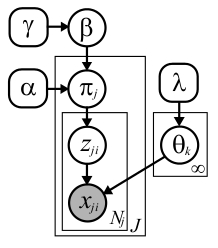
\includegraphics{sb.jpg}\ \ \ \ \ \ \ \ \ \ \ \ \ \ \ \ \ \ \ \ \ \ \ 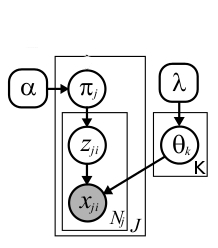
\includegraphics{lda.jpg}\\
Stick-breaking representation for HDP\ \ \ \ \ \ \ \ \ \ \ \ \ \ \ \ \ \ \ \ \ \ \ LDA
\end{center}
\begin{table}[ht]
\begin{minipage}[b]{0.5\linewidth}
{\bf HDP:}\\
$\beta \sim GEM(\gamma)\approx\mathcal{D}(\frac{\gamma}{K})$\\
$\pi_{j} \sim DP(\alpha,\beta)\approx\mathcal{D}(\alpha\beta)$\\
$\theta_{k} \sim H(\lambda)\approx\mathcal{D}(\lambda)$\\
$z_{ji} \sim \mathcal{M}(\pi_{j})$\\
$x_{ji} \sim \mathcal{M}(\theta_{z_{ji}})$\\ 
\end{minipage}
\hspace{0.5cm}
\begin{minipage}[b]{0.5\linewidth}
\begin{center}
{\bf LDA:}\\
$\pi_{j} \sim \mathcal{D}(\alpha)$\\
$\theta_{k} \sim \mathcal{D}(\lambda)$\\
$z_{ji} \sim \mathcal{M}(\pi_{j})$\\
$x_{ji} \sim \mathcal{M}(\theta_{z_{ji}})$\\ 
\end{center}
\end{minipage}
\end{table}
where\\
$\mathcal{D}(.)$: Dirichlet Distribution\\
$\mathcal{M}(.)$: Multinomial Distribution\\
\begin{enumerate}[(A)]
 \item Get $t_{ji}^{*},k_{jt}^{*}$ from ME algorithm in CRF representation and transform it into $\vec z^{*}$ in SB representation
 \item Given $\vec z^{*}$ and $\vec x$, approximate $\vec\theta^{*}$ and $\vec \beta^{*}$ in HDP for LDA evaluation
\begin{enumerate}
\item {\bf $\vec \theta^{*}$}\\
\begin{eqnarray*}
\vec \theta^{*}&=&argmax_{\vec \theta} \ P(\vec \theta|\vec z^{*},\vec x,\lambda)\\
&\sim&argmax_{\vec \theta} \ P(\vec \theta,\vec x|\vec z^{*},\lambda)\\
&=&argmax_{\vec \theta} \ P(\vec x|\vec z^{*},\vec \theta)P(\vec \theta|\lambda)\\
&=&argmax_{\vec \theta} \ [\Pi_{j,i}\mathcal{M}(x_{ji};\theta_{z_{ji}})]\mathcal{D}(\vec \theta;\lambda)\\
&=&argmax_{\vec \theta} \ [\Pi_{j,i}\mathcal{M}(x_{ji};\theta_{z_{ji}})]\mathcal{D}(\vec \theta;\lambda)\\
&=&argmax_{\vec \theta} \ \mathcal{D}(\vec \theta;\lambda+\vec n)\\
&=&(\frac{\lambda+n_{kw}}{W\lambda+\sum_{k}n_{kw})})\\
\end{eqnarray*}
where $n_{kw}$ is the count of number of words w in all restaurants that appear in topic k\\
\item {\bf $\vec \beta^{*}$}
\begin{eqnarray*}
\vec \beta^{*}&=&argmax_{\vec \beta} \ P(\vec \beta|\alpha,\gamma)\\
&=&argmax_{\vec \beta} \ P(\vec \beta,\vec z^{*}|\alpha,\gamma)\\
&=&argmax_{\vec \beta} \ \int P(\vec \beta,\vec z^{*},\vec \pi|\alpha,\gamma)\ d\pi\\
&=&argmax_{\vec \beta} \ [\int P(\vec z^{*}|\vec \pi)P(\vec \pi|\alpha,\vec \beta)\ d\pi]P(\vec \beta|\gamma)\\
&\approx&argmax_{\vec \beta} \ [\int \mathcal{M}(\vec z^{*};\vec \pi)\mathcal{D}(\vec \pi;\alpha\vec \beta)\ d\pi]\mathcal{D}(\vec \beta;\frac{\gamma}{K})\\
&=&argmax_{\vec \beta} \ [(\dfrac{\Pi_{k}\Gamma(\alpha\beta_{k})}{\Gamma(\alpha\vec \beta)})^{J}\Pi_{j}\dfrac{\Gamma(n_{j.}+\alpha\vec \beta)}{\Pi_{k}\Gamma(n_{jk}+\alpha\beta_{k})}][\dfrac{\Pi_{k}\Gamma(\frac{\gamma}{K})}{\Gamma(\gamma)}\Pi_{k}\beta_{k}^{\frac{\gamma}{K}}]\\
\end{eqnarray*}
where $n_{jk}$ is the count of number of words in restaurant j that appear in topic k\\
\end{enumerate}
\item For LDA evaluation, use $\vec\theta^{*}$ for $\theta_{LDA}$ and and $\alpha\vec \beta^{*}$ for $\alpha_{LDA}$\\
(Note that $\vec \beta^{*}$ doesn't have a close form and need to be approximated from constraint nonlinear optimization.)
\end{enumerate}
\end{spacing}
\end{document}

%%%%%%%%%%%%%%%%%%%%%%%%%%%%%%%%%%%%%%%%%%%%%%%%%%%%%%%%%%%%%
